\documentclass[11pt,a4paper]{article}

% ===== Packages =====
\usepackage[utf8]{inputenc}
\usepackage[T1]{fontenc}
\usepackage{amsmath,amssymb,amsfonts}
\usepackage{graphicx}
\usepackage{booktabs}
\usepackage{hyperref}
\usepackage[numbers,sort&compress]{natbib}
\usepackage{subcaption}
\usepackage{siunitx}
\usepackage{adjustbox}
\usepackage{soul}
\usepackage{tikz}
\usetikzlibrary{arrows.meta, positioning, shapes, calc}
\usepackage{longtable}
\usepackage[dvipsnames]{xcolor}
\usepackage[margin=1in]{geometry}
\usepackage{lineno}  % For line numbers during review

% ===== Hyperref Setup =====
\hypersetup{
    colorlinks=true,
    linkcolor=blue,
    citecolor=blue,
    urlcolor=blue
}

% ===== Custom Commands =====
\newcommand{\vect}[1]{\mathbf{#1}}
\newcommand{\matr}[1]{\mathbf{#1}}

% ===== Title and Authors =====
\title{Sequential RNN Deep Networks for Predicting UV Absorption Properties of Organic Molecules}

\author{
    Umesh Arampath$^{1,*}$ \\[0.5em]
    \small $^1$Department of Mathematics, University of Iowa, Iowa City, USA \\
    \small $^2$Midwest Bioprocessing Center, Illinois, USA \\[0.3em]
    \small $^*$Corresponding author: uarampath@mwbioprocessing.com
}

\date{}

\begin{document}

\maketitle

% ===== Abstract =====
\begin{abstract}
Accurate prediction of UV absorption properties is essential for the rational design of molecules
targeting applications in sunscreen formulation, pharmaceutical development, and optoelectronic
materials. However, predicting the maximum absorption wavelength ($\lambda_{\max}$) of organic
molecules remains challenging due to the complex dependence of UV absorption on molecular
electronic structure and solute--solvent interactions. In this work, we present a deep learning
framework based on bidirectional Gated Recurrent Unit (BiGRU) networks that predicts
$\lambda_{\max}$ directly from SMILES string representations of organic molecules. We leverage
two comprehensive experimental UV/Vis absorption databases comprising 18,755
solute--solvent pairs across more than 15,000 unique organic chromophores measured in hundreds of solvent
conditions. A key contribution is the integration
of solvent information through a sequence concatenation strategy,
where SMILES representations of both the solute and solvent are combined into a single input
sequence with special delimiter tokens. Using rigorous stratified 5-fold cross-validation with proper train/validation/test separation, the solvent-aware BiGRU model achieves RMSE~$= 36.45 \pm 1.12$~nm ($R^2 = 0.884$), improving over the solute-only baseline (RMSE~$= 37.85$~nm). Classical Random Forest models on Morgan fingerprints achieve RMSE~$= 32.18 \pm 1.74$~nm on this dataset. We benchmark our approach against four external datasets with published baselines: on Deep4Chem, our BiGRU achieves RMSE~$= 27.07$~nm, within 2\% of the published GCNN result (26.6~nm), while cross-dataset evaluation on nablaColors reveals fundamental limitations of 1D SMILES models versus 3D geometry-aware approaches. We further validate our models on ICH~S10 photosafety classification using a reconstructed Reaxys dataset of 74,784 compounds. Experimental validation on commercial UV-absorbing compounds demonstrates prediction errors of 5--11~nm, establishing sequential RNN architectures with solvent-aware encoding as an effective and
computationally efficient approach for predicting UV absorption properties.
\end{abstract}

\noindent\textbf{Keywords:} machine learning; molecular design; deep learning; SMILES; property prediction

\section{Introduction}

\begin{figure}[H]
  \centering
  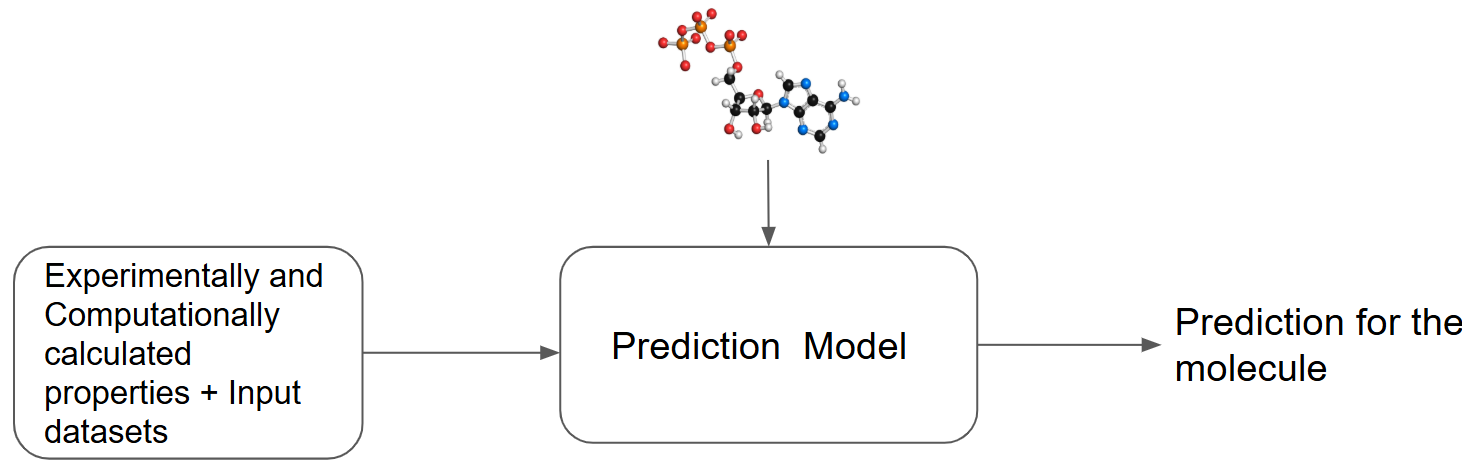
\includegraphics[scale=0.5]{p_1.png}
  \caption{Schematic overview of the predictive modeling process  }
  \label{fig:overview}
\end{figure}

Molecular property prediction is a fundamental task in computational chemistry and drug discovery, aiming to estimate physicochemical, biological, or pharmacological properties of molecules directly from their structural representations \cite{wuMoleculeNetBenchmarkMolecular2018}. Traditional approaches rely on handcrafted molecular descriptors or fingerprints, which require domain expertise and may not capture all relevant structural features.

Deep learning approaches have emerged as powerful alternatives, capable of learning molecular representations directly from raw structural data. Among various molecular representations, the Simplified Molecular Input Line Entry System (SMILES) \cite{SMILESChemicalLanguage} has gained widespread adoption due to its simplicity and ability to represent complex molecular structures as linear strings.

Recurrent Neural Networks (RNNs), particularly variants designed to handle long-range dependencies such as Long Short-Term Memory (LSTM) and Gated Recurrent Units (GRU), are well-suited for processing SMILES strings as sequential data. These architectures can capture the inherent sequential nature of SMILES notation and learn meaningful molecular representations for property prediction tasks.

This work presents a comprehensive framework for predicting molecular UV absorption properties using bidirectional GRU networks operating on SMILES representations. We discuss the SMILES encoding scheme, RNN architectures, and our complete model pipeline for predicting molecular properties.

\subsection{Molecular Representation Methods}

\begin{figure}[H]
  \centering
  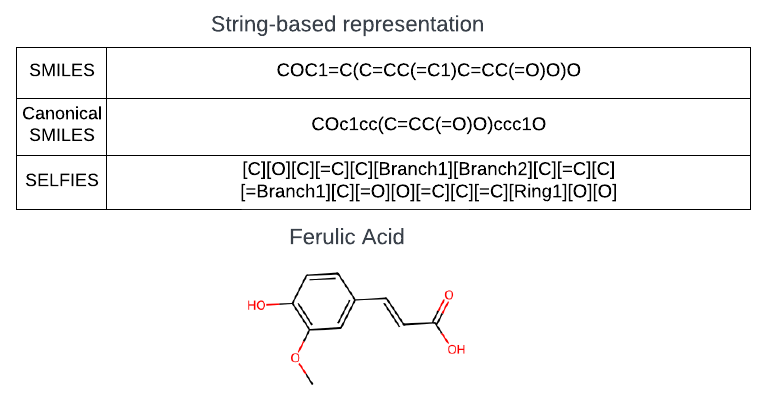
\includegraphics[scale=1]{3.png}
  \caption{String Based Representations of Ferulic Acid  }
  \label{fig:ferulic_representations}
\end{figure}


Deep learning approaches in the chemistry domain depend on how molecular data is represented. The Simplified Molecular Input Line Entry System (SMILES) is a ``chemical language'' \cite{weiningerSMILESChemicalLanguage1988} that encodes structural information of a chemical into a compact text representation. By mapping atoms to characters and bonds to punctuation, SMILES transforms the molecule structure of a molecule into a linear sequence. For example, c and C denote aromatic and aliphatic carbons respectively. Special characters like ‘=’ denote the type of bonds (connections between atoms). Rings are denoted by encapsulating numbers, and side chains by round brackets. 

The main advantage of the SMILES representation is its compatibility with deep learning architectures developed for Natural Language Processing (NLP). By treating molecules as text, we can directly leverage sequence processing models such as Recurrent Neural Networks (RNNs), Long Short-Term Memory (LSTM) networks, and Transformers to train the deep learning models.

Therefore, datasets with SMILES representation of molecules were used in this project, as this aligns with our objective of developing computationally efficient property prediction models.

\begin{figure}[H]
  \centering
  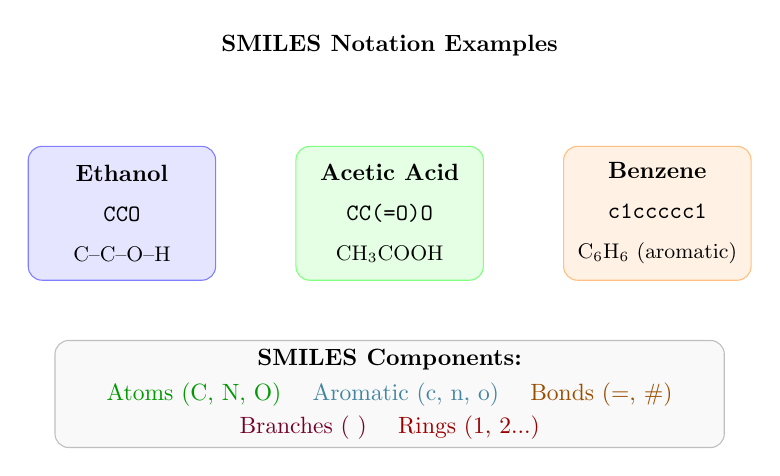
\begin{tikzpicture}[scale=0.85, transform shape]
    
    % Title
    \node[font=\bfseries] at (0, 4) {SMILES Notation Examples};
    
    % Example 1: Ethanol
    \begin{scope}[shift={(-4, 1.5)}]
      \node[draw=blue!50, rounded corners=5pt, fill=blue!10, 
            minimum width=2.8cm, minimum height=2cm, align=center] {
        \textbf{Ethanol}\\[5pt]
        \texttt{CCO}\\[5pt]
        \small C--C--O--H
      };
    \end{scope}
    
    % Example 2: Acetic Acid
    \begin{scope}[shift={(0, 1.5)}]
      \node[draw=green!50, rounded corners=5pt, fill=green!10, 
            minimum width=2.8cm, minimum height=2cm, align=center] {
        \textbf{Acetic Acid}\\[5pt]
        \texttt{CC(=O)O}\\[5pt]
        \small CH$_3$COOH
      };
    \end{scope}
    
    % Example 3: Benzene
    \begin{scope}[shift={(4, 1.5)}]
      \node[draw=orange!50, rounded corners=5pt, fill=orange!10, 
            minimum width=2.8cm, minimum height=2cm, align=center] {
        \textbf{Benzene}\\[5pt]
        \texttt{c1ccccc1}\\[5pt]
        \small C$_6$H$_6$ (aromatic)
      };
    \end{scope}
    
    % Legend - two rows
    \node[draw=gray!50, rounded corners=5pt, fill=gray!5, 
          minimum width=10cm, minimum height=1.6cm, align=center] at (0, -1.2) {
      \textbf{SMILES Components:}\\[3pt]
      \textcolor{green!60!black}{Atoms (C, N, O)} \quad
      \textcolor{cyan!60!black}{Aromatic (c, n, o)} \quad
      \textcolor{orange!60!black}{Bonds (=, \#)}\\[2pt]
      \textcolor{purple!60!black}{Branches ( )} \quad
      \textcolor{red!60!black}{Rings (1, 2...)}
    };
    
  \end{tikzpicture}
  \caption{Examples of SMILES notation for common molecules. SMILES encodes molecular structures as linear strings using specific symbols for atoms, bonds, branches, and ring closures.}
  \label{fig:smiles_examples}
\end{figure}

\subsection{Data Challenges}

The performance of data-driven models in chemistry is highly dependent on data quality and domain specificity. For UV absorption prediction, the primary challenge is that $\lambda_{max}$ is \textbf{measured with respect to a solvent}. Chromophores (carbonyl, nitro, azo, and other functional groups) are responsible for UV-Vis absorption, and their interaction with the solvent environment heavily influences the observed $\lambda_{max}$ \cite{koplikUltravioletVisibleSpectrometry, clarkWhatCausesMolecules2013}. Therefore, the corresponding solvent information and the solute molecule must be considered together. These solvents are not uniform across datasets or even within the same dataset, presenting a significant challenge for model development. Considerable data engineering effort was required to filter, process, clean, and standardize the source databases into a uniform SMILES-based format suitable for model training.

\section{Related Work}


The Simplified Molecular-Input Line-Entry System (SMILES) provides a text-based representation of molecules that enables the application of natural language processing (NLP) techniques to chemical structures \citep{weiningerSMILESChemicalLanguage1988}. As SMILES strings are sequential and composed of characters, methods inspired by NLP such as word embeddings and recurrent neural networks have been extensively explored for molecular property prediction \citep{gohSMILES2VecInterpretableGeneralPurpose2018}.

Early deep learning approaches for SMILES-based property prediction employed recurrent neural networks (RNNs). \citet{xuSeq2seqFingerprintUnsupervised2017} introduced Seq2seq fingerprint, which learns molecular embeddings using encoder-decoder RNN architectures in an unsupervised manner. Long Short-Term Memory (LSTM) and Gated Recurrent Unit (GRU) networks have gained widespread adoption for processing SMILES sequences due to their ability to capture long-range dependencies \citep{GeneratingFocusedMolecule}. \citet{gohSMILES2VecInterpretableGeneralPurpose2018} proposed SMILES2vec, an interpretable deep neural network that processes SMILES strings for predicting chemical properties. Bidirectional LSTM architectures have shown particular promise, demonstrating that BiLSTM models with attention mechanisms achieve competitive performance in predicting aqueous solubility and partition coefficients.

Convolutional neural networks (CNNs) have also been applied to SMILES-based prediction. \citet{hiroharaConvolutionalNeuralNetwork2018a} proposed SCFP (SMILES-based Convolutional Fingerprint), which processes one-hot encoded SMILES vectors using convolutional layers. 

The introduction of Transformer architectures has significantly advanced molecular property prediction. \citet{wangSMILESBERTLargeScale2019} developed SMILES-BERT, adapting the BERT framework for molecular representations through masked token prediction on large-scale unlabeled SMILES data. \citet{honda2019smiles} proposed SMILES Transformer for pre-trained molecular fingerprints, demonstrating effectiveness in low-data drug discovery scenarios. 

Recognizing that different molecular representations capture complementary information, hybrid approaches have emerged. GraSeq \citep{guoGraSeqGraphSequence2020} combines SMILES sequences with molecular graphs using LSTM and graph neural networks to capture both sequential and topological information. MTBG \citep{liuPredictionMolecularToxicity2023} integrates SMILES processing via BiGRU with molecular graph embeddings using GraphSAGE for toxicity prediction.

\subsection{Comparative Studies: RNN vs Transformer}

\citet{chenMolecularLanguageModels2023} conducted a systematic comparison of RNN-based and Transformer-based language models across three molecular generation tasks of varying complexity. Their findings revealed that the optimal architecture choice depends on the characteristics of the target property. Specifically, RNNs demonstrated superior performance on tasks where molecular properties are determined by local structural features, while Transformers excelled when global molecular architecture and long-range dependencies were paramount.

Several factors support the selection of RNNs for UV absorption prediction:

\textbf{Local Feature Dependence.} UV-Vis absorption maxima ($\lambda_{max}$) are primarily governed by chromophoric groups and their immediate electronic environments. The $\pi \rightarrow \pi^*$ and $n \rightarrow \pi^*$ transitions responsible for UV absorption arise from localized conjugated systems, carbonyl groups, and aromatic rings. \citet{chenMolecularLanguageModels2023} demonstrated that RNNs outperform Transformers on properties such as logP, which are computed as sums of atomic contributions, a paradigm analogous to how electronic transitions depend on local chromophore contributions. The partition coefficient logP shares computational similarities with UV absorption, as both properties can be decomposed into contributions from molecular substructures.

\textbf{Moderate Sequence Lengths.} The molecules in our dataset, comprising sunscreen compounds and phenolic acids, exhibit moderate molecular weights and SMILES sequence lengths typically ranging from 30 to 80 tokens. \citet{chenMolecularLanguageModels2023} found that RNNs perform optimally in this regime, with performance degradation occurring primarily for large molecules exceeding 100 heavy atoms. The Transformer's advantage in capturing long-range dependencies becomes relevant only for sequences substantially longer than those in our dataset.

\textbf{Sequential Structure Encoding.} SMILES strings encode molecular structure in a manner where adjacent tokens often represent chemically connected atoms. RNNs naturally capture these local adjacency relationships through their recurrent hidden state updates. For chromophore identification, the sequential processing of RNNs aligns well with tracing conjugation pathways through the molecular graph as encoded in the SMILES representation.

\textbf{Computational Efficiency.} For our dataset size and sequence lengths, RNNs offer favorable computational characteristics. The quadratic attention complexity of Transformers with respect to sequence length provides no advantage for moderate-length SMILES strings, while RNNs achieve comparable or superior performance with linear complexity.

It should be noted that Transformers may offer advantages for related tasks involving larger molecules or properties requiring global structural awareness. However, for the specific application of predicting UV absorption wavelengths in small to medium-sized organic chromophores, the empirical evidence and theoretical considerations favor RNN-based architectures.


\section{Methods}

\subsection{Dataset Description and Preparation}


The accurate prediction of UV absorption properties for small molecules has significant implications for industrial applications, including pharmaceutical development, sunscreen formulation, and optoelectronic materials design. To build a robust machine learning model capable of predicting UV absorption maxima ($\lambda_{max}$) for organic compounds, we identified and combined two comprehensive experimental databases from the literature. The selection criteria prioritized datasets with: (1) experimentally validated absorption measurements, (2) standardized SMILES representations for molecular structures, (3) documented solvent information, and (4) sufficient size and chemical diversity for training deep learning models.

\subsection{Dataset 1: Experimental Database of Optical Properties of Organic Compounds}

The first dataset employed in this study is the Experimental Database of Optical Properties of Organic Compounds, developed by Joung et al. \cite{joungExperimentalDatabaseOptical2020}. This database was specifically curated to facilitate data-driven chemistry applications using machine learning approaches. The dataset was constructed by systematically collecting optical properties of organic compounds from previously published literature sources.

The database comprises 20,236 data points spanning 7,016 unique organic chromophores measured in 365 different solvents or in the solid state. The optical properties recorded are derived from absorption and emission spectra as reported in the original publications. Table~\ref{tab:dataset1_format} describes the data fields available in this database.

\begin{table}[H]
\centering
\caption{Data fields in the Experimental Database of Optical Properties of Organic Compounds.}
\label{tab:dataset1_format}
\begin{tabular}{ll}
\toprule
\textbf{Field} & \textbf{Description} \\
\midrule
SMILES & Canonical SMILES representation of the molecule \\
Solvent & Solvent used for measurement \\
Absorption max (nm) & Wavelength of maximum absorption \\
Emission max (nm) & Wavelength of maximum emission \\
Quantum yield & Fluorescence quantum yield \\
Extinction coefficient & Molar extinction coefficient \\
Reference & Original literature source \\
\bottomrule
\end{tabular}
\end{table}

The comprehensive coverage of solvent conditions in this dataset makes it particularly valuable for our solvent-aware prediction approach, as it enables the model to learn solvatochromic effects across a diverse range of solute-solvent combinations.

\subsection{Dataset 2: Comparative Dataset of UV/Vis Absorption Spectra}

The second dataset utilized is the Comparative Dataset of Experimental and Computational Attributes of UV/Vis Absorption Spectra, developed by Beard et al. \cite{beardComparativeDatasetExperimental2019}. This database was auto-generated through systematic extraction from the literature and contains 18,309 records of experimentally determined UV/Vis absorption maxima along with associated extinction coefficients where available.

The dataset encompasses 8,488 unique compounds, with a subset of 5,380 compounds containing both experimental and computational data. The database is provided in multiple formats including MongoDB, CSV, and JSON, facilitating integration with various programming environments such as Python, R, Java, and MATLAB.
\begin{table}[H]
\centering
\caption{Summary of Dataset 2 characteristics.}
\label{tab:dataset2_summary}
\begin{tabular}{ll}
\toprule
\textbf{Attribute} & \textbf{Value} \\
\midrule
Total records & 18,309 \\
Unique compounds & 8,488 \\
Compounds with experimental + computational data & 5,380 \\
Available formats & MongoDB, CSV, JSON \\
Primary properties & $\lambda_{max}$, extinction coefficient \\
\bottomrule
\end{tabular}
\end{table}

To maximize the training data available for our deep learning model, we combined both datasets.

\subsection{Neural Network Architecture}

Recurrent Neural Networks (RNNs) are designed to process sequential data by maintaining a hidden state that captures information from previous time steps. One of the main challenges in applying RNN networks is designing an appropriate network architecture. The optimal combination of various network parameters (types and sizes of network layers, activation and optimization functions, learning and dropout rates, and the optimal way to encode the training data into vectorized form required by the network) requires some trial and error. There are no general rules for designing the optimal architecture; one has to experiment with different architectures and parameters.

This section presents our best-performing model architecture, as well as alternative architectures evaluated, for SMILES-based molecular property prediction. The model integrates embedding, bidirectional GRU layers, and fully connected layers.

To use SMILES strings as input to neural networks, they must be converted to numerical representations through the following steps:

\begin{enumerate}
    \item \textbf{Tokenization}: Split the SMILES string into individual tokens (characters or multi-character symbols like \texttt{Cl}, \texttt{Br}).
    \item \textbf{Vocabulary Mapping}: Map each unique token to an integer index.
    \item \textbf{Padding}: Pad sequences to a fixed maximum length $T_{\max}$ for batch processing.
    \item \textbf{Embedding}: Convert integer indices to dense vector representations.
\end{enumerate}

\begin{figure}[H]
  \centering
  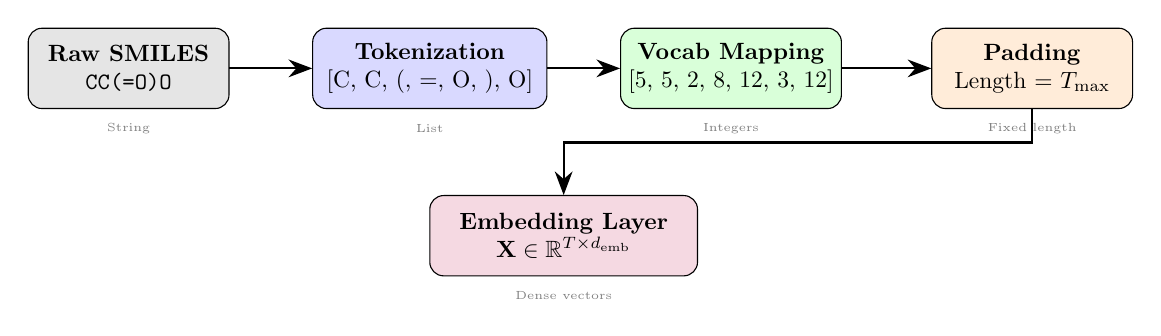
\begin{tikzpicture}[scale=0.85, transform shape,
    box/.style={draw, rounded corners=5pt, minimum height=1.2cm, align=center},
    arrow/.style={-{Stealth[length=3mm]}, thick}
  ]
    
    % Stage 1: Raw SMILES
    \node[box, fill=gray!20, minimum width=3cm] (raw) at (-6, 0) {
      \textbf{Raw SMILES}\\
      \texttt{CC(=O)O}
    };
    
    % Stage 2: Tokenization
    \node[box, fill=blue!15, minimum width=3.5cm] (token) at (-1.5, 0) {
      \textbf{Tokenization}\\
      {[C, C, (, =, O, ), O]}
    };
    
    % Stage 3: Vocabulary Mapping
    \node[box, fill=green!15, minimum width=3cm] (vocab) at (3, 0) {
      \textbf{Vocab Mapping}\\
      {[5, 5, 2, 8, 12, 3, 12]}
    };
    
    % Stage 4: Padding
    \node[box, fill=orange!15, minimum width=3cm] (pad) at (7.5, 0) {
      \textbf{Padding}\\
      Length = $T_{\max}$
    };
    
    % Stage 5: Embedding (below)
    \node[box, fill=purple!15, minimum width=4cm] (embed) at (0.5, -2.5) {
      \textbf{Embedding Layer}\\
      $\mathbf{X} \in \mathbb{R}^{T \times d_{\text{emb}}}$
    };
    
    % Arrows
    \draw[arrow] (raw) -- (token);
    \draw[arrow] (token) -- (vocab);
    \draw[arrow] (vocab) -- (pad);
    \draw[arrow] (pad.south) -- ++(0, -0.5) -| (embed.north);
    
    % Dimension annotations
    \node[font=\tiny, gray] at (-6, -0.9) {String};
    \node[font=\tiny, gray] at (-1.5, -0.9) {List};
    \node[font=\tiny, gray] at (3, -0.9) {Integers};
    \node[font=\tiny, gray] at (7.5, -0.9) {Fixed length};
    \node[font=\tiny, gray] at (0.5, -3.4) {Dense vectors};
    
  \end{tikzpicture}
  \caption{SMILES processing pipeline for neural network input. Raw SMILES strings are tokenized, mapped to integers via a vocabulary, padded to fixed length, and embedded into dense vector representations.}
  \label{fig:smiles_pipeline}
\end{figure}

\tikzstyle{startstop} = [rectangle, rounded corners, minimum width=3cm, minimum height=1cm,text centered, draw=black]
\tikzstyle{process} = [rectangle, minimum width=3cm, minimum height=1cm, text centered, draw=black]
\tikzstyle{arrow} = [thick,->,>=stealth]


The model consists of the following components:

\begin{enumerate}
    \item \textbf{Embedding Layer}: Maps tokenized SMILES characters to dense vectors of dimension 50.
    
    \item \textbf{Bidirectional GRU Layer 1}: Processes embedded sequences bidirectionally with 128 hidden units per direction, outputting 128-dimensional hidden states.
    
    \item \textbf{Bidirectional GRU Layer 2}: Further processes the sequence with another BiGRU layer (128 units per direction), capturing higher-level sequential patterns.
    
    \item \textbf{Global Average Pooling}: Aggregates variable-length sequences into fixed-length vectors by averaging across time steps.
    
    \item \textbf{Dense Layer}: A fully connected layer with 128 units and ReLU activation transforms the pooled representation.
    
    \item \textbf{Dropout Layer}: Applies dropout with rate 0.2 for regularization.
    
    \item \textbf{Output Layer}: A linear layer produces the final property prediction.
\end{enumerate}

% ============================================================================
% FIGURE: Complete Model Architecture
% ============================================================================
\begin{figure}[H]
  \centering
  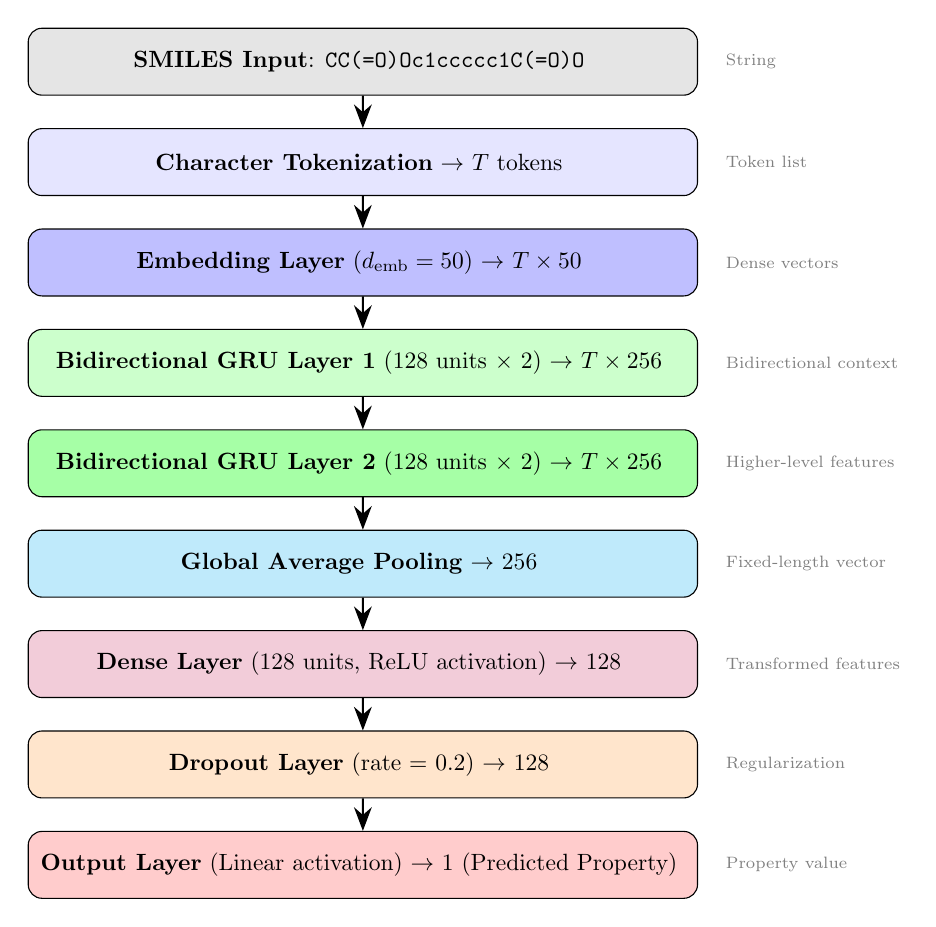
\begin{tikzpicture}[scale=0.85, transform shape,
    layer/.style={draw, rounded corners=5pt, minimum width=10cm, minimum height=1cm, align=center},
    arrow/.style={-{Stealth[length=3mm]}, thick}
  ]
    
    % Input
    \node[layer, fill=gray!20] (input) at (0, 0) {
      \textbf{SMILES Input}: \texttt{CC(=O)Oc1ccccc1C(=O)O}
    };
    
    % Tokenization
    \node[layer, fill=blue!10] (token) at (0, -1.5) {
      \textbf{Character Tokenization} $\rightarrow$ $T$ tokens
    };
    
    % Embedding
    \node[layer, fill=blue!25] (embed) at (0, -3) {
      \textbf{Embedding Layer} ($d_{\text{emb}} = 50$) $\rightarrow$ $T \times 50$
    };
    
    % BiGRU 1
    \node[layer, fill=green!20] (bigru1) at (0, -4.5) {
      \textbf{Bidirectional GRU Layer 1} (128 units $\times$ 2) $\rightarrow$ $T \times 256$
    };
    
    % BiGRU 2
    \node[layer, fill=green!35] (bigru2) at (0, -6) {
      \textbf{Bidirectional GRU Layer 2} (128 units $\times$ 2) $\rightarrow$ $T \times 256$
    };
    
    % Global Pooling
    \node[layer, fill=cyan!25] (pool) at (0, -7.5) {
      \textbf{Global Average Pooling} $\rightarrow$ 256
    };
    
    % Dense
    \node[layer, fill=purple!20] (dense) at (0, -9) {
      \textbf{Dense Layer} (128 units, ReLU activation) $\rightarrow$ 128
    };
    
    % Dropout
    \node[layer, fill=orange!20] (dropout) at (0, -10.5) {
      \textbf{Dropout Layer} (rate = 0.2) $\rightarrow$ 128
    };
    
    % Output
    \node[layer, fill=red!20] (output) at (0, -12) {
      \textbf{Output Layer} (Linear activation) $\rightarrow$ 1 (Predicted Property)
    };
    
    % Arrows
    \draw[arrow] (input) -- (token);
    \draw[arrow] (token) -- (embed);
    \draw[arrow] (embed) -- (bigru1);
    \draw[arrow] (bigru1) -- (bigru2);
    \draw[arrow] (bigru2) -- (pool);
    \draw[arrow] (pool) -- (dense);
    \draw[arrow] (dense) -- (dropout);
    \draw[arrow] (dropout) -- (output);
    
    % Dimension annotations (right side)
    \node[font=\scriptsize, gray, right] at (5.3, 0) {String};
    \node[font=\scriptsize, gray, right] at (5.3, -1.5) {Token list};
    \node[font=\scriptsize, gray, right] at (5.3, -3) {Dense vectors};
    \node[font=\scriptsize, gray, right] at (5.3, -4.5) {Bidirectional context};
    \node[font=\scriptsize, gray, right] at (5.3, -6) {Higher-level features};
    \node[font=\scriptsize, gray, right] at (5.3, -7.5) {Fixed-length vector};
    \node[font=\scriptsize, gray, right] at (5.3, -9) {Transformed features};
    \node[font=\scriptsize, gray, right] at (5.3, -10.5) {Regularization};
    \node[font=\scriptsize, gray, right] at (5.3, -12) {Property value};
    
  \end{tikzpicture}
  \caption{Complete model architecture for SMILES-based molecular property prediction. The model processes SMILES strings through embedding, stacked bidirectional GRU layers, global average pooling, and fully connected layers with dropout regularization.}
  \label{fig:complete_architecture}
\end{figure}

\tikzstyle{startstop} = [rectangle, rounded corners, minimum width=3cm, minimum height=1cm, text centered, draw=black]
\tikzstyle{process} = [rectangle, minimum width=3cm, minimum height=1cm, text centered, draw=black]
\tikzstyle{arrow} = [thick,->,>=stealth]

\begin{figure}[H]
\centering

% Top row - two figures side by side
\begin{minipage}[t]{0.48\textwidth}
\centering
\begin{tikzpicture}[node distance=1.5cm, scale=0.85, transform shape]
\node (start) [startstop] {Embedding Layer - 50};
\node (pro1) [process, below of=start] {Bidirectional GRU Layer - 128};
\node (pro2) [process, below of=pro1] {Bidirectional GRU Layer - 128};
\node (pro3) [process, below of=pro2] {Dense Layer (ReLU) - 128};
\node (pro4) [process, below of=pro3] {Dropout Layer - 0.2};
\node (pro5) [process, below of=pro4] {Dense Layer (Linear) - 128};
\draw [arrow] (start) -- (pro1);
\draw [arrow] (pro1) -- (pro2);
\draw [arrow] (pro2) -- (pro3);
\draw [arrow] (pro3) -- (pro4);
\draw [arrow] (pro4) -- (pro5);
\end{tikzpicture}
\subcaption{BiGRU Architecture}
\label{fig:bigru}
\end{minipage}
\hfill
\begin{minipage}[t]{0.48\textwidth}
\centering
\begin{tikzpicture}[node distance=1.5cm, scale=0.85, transform shape]
\node (start) [startstop] {Embedding Layer - 50};
\node (pro1) [process, below of=start] {Bidirectional LSTM Layer - 128};
\node (pro2) [process, below of=pro1] {Bidirectional LSTM Layer - 128};
\node (pro3) [process, below of=pro2] {Dense Layer (ReLU) - 128};
\node (pro4) [process, below of=pro3] {Dropout Layer - 0.2};
\node (pro5) [process, below of=pro4] {Dense Layer (Linear) - 128};
\draw [arrow] (start) -- (pro1);
\draw [arrow] (pro1) -- (pro2);
\draw [arrow] (pro2) -- (pro3);
\draw [arrow] (pro3) -- (pro4);
\draw [arrow] (pro4) -- (pro5);
\end{tikzpicture}
\subcaption{BiLSTM Architecture}
\label{fig:bilstm}
\end{minipage}

\vspace{1cm}

% Bottom row - one figure centered
\begin{minipage}[t]{0.5\textwidth}
\centering
\begin{tikzpicture}[node distance=1.5cm, scale=0.85, transform shape]
\node (start) [startstop] {Embedding Layer - 50};
\node (pro1) [process, below of=start] {Conv1D Layer - 192, 3};
\node (pro2) [process, below of=pro1] {Bidirectional GRU Layer - 128};
\node (pro3) [process, below of=pro2] {Bidirectional GRU Layer - 128};
\node (pro4) [process, below of=pro3] {Dense Layer (ReLU) - 128};
\node (pro5) [process, below of=pro4] {Dropout Layer - 0.2};
\node (pro6) [process, below of=pro5] {Dense Layer (Linear) - 128};
\draw [arrow] (start) -- (pro1);
\draw [arrow] (pro1) -- (pro2);
\draw [arrow] (pro2) -- (pro3);
\draw [arrow] (pro3) -- (pro4);
\draw [arrow] (pro4) -- (pro5);
\draw [arrow] (pro5) -- (pro6);
\end{tikzpicture}
\subcaption{CNN-BiGRU Architecture}
\label{fig:cnn-bigru}
\end{minipage}

\caption{Neural network architectures tested for SMILES-based regression predictions of UV absorption max: (a) Bidirectional GRU, (b) Bidirectional LSTM, and (c) CNN-Bidirectional GRU hybrid.}
\label{fig:architectures}
\end{figure}

\subsection{Integration of Solvent Information into the Model}

UV absorption is inherently a system-dependent property that depends not only on the molecular structure of the solute but also critically on the nature of the solvent. Solvatochromic shifts---changes in $\lambda_{\max}$ arising from solute--solvent interactions such as hydrogen bonding, dipole--dipole coupling, and dielectric stabilization of excited states---can reach tens of nanometers \cite{reichardt2011solvents}. Traditional machine learning approaches for spectral property prediction often neglect explicit solvent information, treating $\lambda_{\max}$ as an intrinsic molecular property. However, practical applications in pharmaceutical development, sunscreen formulation, and materials design require accurate predictions across diverse solvent systems.


Several strategies have been proposed for incorporating solvent information into deep learning models for property prediction:

\paragraph{Descriptor-Based Approaches.} Traditional methods concatenate handcrafted molecular descriptors of the solute with solvent descriptors or physical properties such as dielectric constant, dipole moment, and hydrogen bond donor/acceptor counts \cite{lusci2013deep, boobier2020machine}. While effective, these approaches require feature engineering and may not capture all relevant molecular interactions.


\paragraph{Sequence Concatenation.} An alternative approach involves concatenating the SMILES representations of solute and solvent into a single input sequence, separated by a special delimiter token \cite{schwaller2019molecular, irwin2022chemformer}. This method leverages the sequential processing capabilities of recurrent neural networks or transformers to implicitly learn solute-solvent interactions.

In this work, we adopt a sequence concatenation approach that integrates solvent information directly into the SMILES input representation. The concatenated sequence takes the form:

\begin{equation}
    S_{input} = \texttt{!} \oplus S_{molecule} \oplus \texttt{|} \oplus S_{solvent} \oplus \texttt{\#}
\end{equation}

\noindent where $S_{molecule}$ and $S_{solvent}$ represent the SMILES strings of the solute molecule and solvent, respectively, and $\oplus$ denotes string concatenation. Three special tokens are introduced:

\begin{itemize}
    \item \texttt{!} (Start token): Marks the beginning of the input sequence
    \item \texttt{|}  (Separator token): Delineates the boundary between solute and solvent
    \item \texttt{\#} (End token): Signals the termination of the input sequence
\end{itemize}

For example, acetic acid (CC(=O)O) in ethanol (CCO) would be represented as:

\begin{center}
    \texttt{!CC(=O)O|CCO\#}
\end{center}

This representation is then processed through the tokenization pipeline described below, where each character or multi-character token (e.g., Cl, Br) is mapped to an integer index and subsequently embedded into a continuous vector space.


\begin{figure}[H]
    \centering
    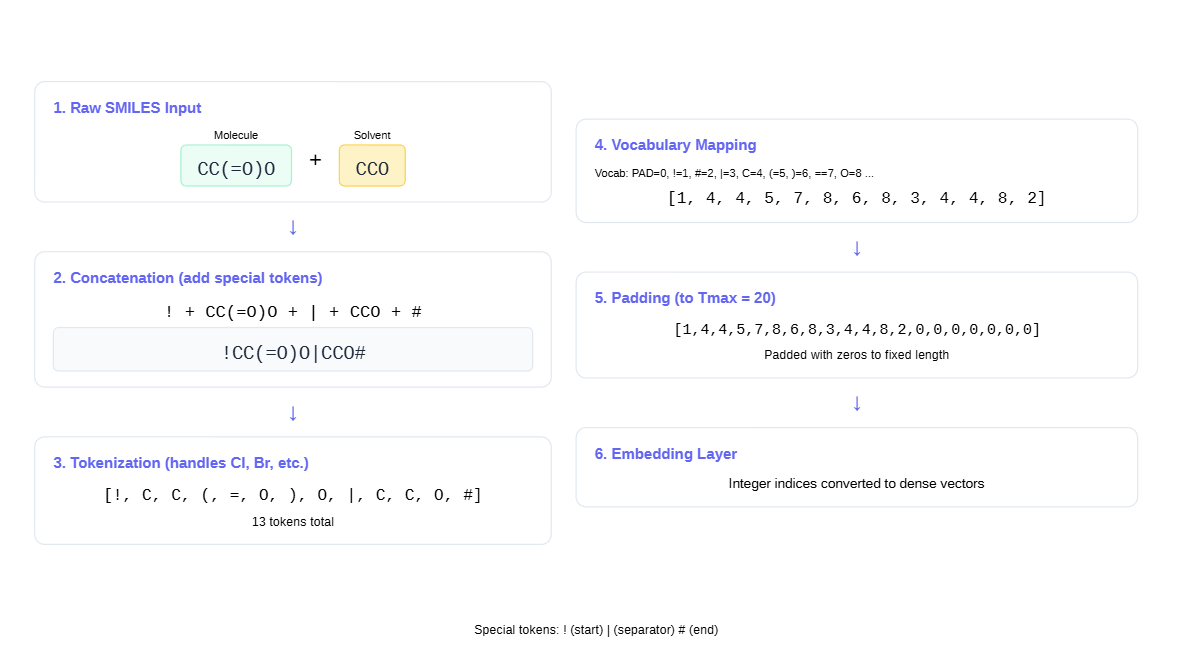
\includegraphics[width=\textwidth]{solvent_to_model.png}
    \caption{Molecule-Solvent concatenation example }
    \label{fig:example}
\end{figure}

The proposed concatenation strategy offers several advantages over alternative methods.

\paragraph{End-to-End Learning.} By encoding both solute and solvent within a single sequence, the model can learn representations that capture solute-solvent interactions directly from data without requiring explicit feature engineering. The recurrent architecture processes the concatenated sequence sequentially.

\paragraph{Unified Vocabulary.} Since both solute and solvent are represented using SMILES notation, they share a common tokenization vocabulary. This eliminates the need for separate encoding schemes and allows the embedding layer to learn unified representations of chemical tokens regardless of whether they appear in the solute or solvent context.



\subsection{Training Configuration}

The model was implemented using TensorFlow 2.20 and Keras with mixed-precision (float16) training. SMILES strings were tokenized at the character level using a vocabulary of 57 unique tokens and padded to a maximum sequence length of 650. The two source databases total over 38,000 records; after merging, removing duplicates, and filtering for non-null $\lambda_{\max}$ values, the final dataset comprised 18,755 solute--solvent pairs.

Model performance was evaluated using stratified 5-fold cross-validation with a 64/16/20 train/validation/test split. Stratification was performed on solvent identity to ensure each fold contains representative proportions of the 20 most common solvents. Within each fold, 80\% of the data was allocated for training and validation (split further into 80/20), with the remaining 20\% held out as the test set. The validation set was used exclusively for early stopping, ensuring no information leakage from the test set during model selection. The model was optimized using RMSprop (learning rate $= 0.001$, $\rho = 0.9$, $\epsilon = 10^{-8}$) with mean absolute error (MAE) as the loss function. Training proceeded with a batch size of 32 for up to 250 epochs, with early stopping (patience = 25 epochs, $\delta_{\min} = 10^{-5}$) restoring the best weights. The model contains approximately 470,000 trainable parameters and was trained on a single NVIDIA RTX 4090 GPU.

\subsection{Baseline Models}

To contextualize the performance of the BiGRU architecture, we evaluated two classical machine learning baselines using Morgan circular fingerprints \cite{morganGenerationMachineSorted1965} as molecular representations:

\paragraph{Random Forest (RF).} We trained Random Forest regressors with 500 estimators on 2048-bit Morgan fingerprints (radius~$= 2$). For solvent-aware models, the solute and solvent fingerprints were concatenated into a 4096-dimensional feature vector. We evaluated models trained with both mean squared error (MSE) and mean absolute error (MAE) loss functions.

\paragraph{XGBoost.} Gradient-boosted tree models were trained with 500 estimators, maximum depth of 6, and learning rate of 0.1, using the same fingerprint representation as the RF models. Both MSE and MAE objectives were evaluated.

\section{External Validation Datasets}
\label{sec:datasets}

To assess the generalizability of our approach beyond the primary Joung+Beard dataset, we benchmarked our BiGRU model and Random Forest baseline against published results on several independent UV absorption datasets. Each dataset was processed using the same split protocol reported by the original authors, enabling direct comparison with their published metrics.

\subsection{Deep4Chem (Joung et al., 2020)}

The Deep4Chem dataset \cite{joungExperimentalDatabaseOptical2020} is the publicly available version of our Dataset~1, distributed via Figshare. It contains approximately 20,000 absorption records for organic chromophores in various solvents. Joung et al.\ reported a graph convolutional neural network (GCNN) achieving RMSE~$= 26.6$~nm using an 80/10/10 random train/validation/test split. We replicated this exact split protocol for direct comparison.

\subsection{Jung et al.\ (2024)}

Jung et al.\ \cite{jung2024} assembled a dataset of approximately 26,000 UV/Vis absorption records from multiple literature sources and trained a gradient-boosted feature selection (GBFS) ensemble model, reporting RMSE~$= 32.2$~nm. Their published protocol uses a 72/18/10 random split. We evaluated our model using both this random split and a more challenging Bemis--Murcko scaffold split \cite{bemisMurckoPropertiesKnown1996} (80/10/10) to assess generalization to structurally novel scaffolds.

\subsection{nablaColors (Potapov, 2026)}

The nablaColors dataset \cite{potapov2026nablacolors} comprises 24,567 absorption records with 3D-optimized molecular geometries. The state-of-the-art UniProp model \cite{uniprop2025}, a 3D graph neural network with 27.7 million parameters, achieves MAE~$= 15.97$~nm using the authors' precomputed scaffold-based splits. This dataset provides a challenging benchmark for evaluating the limitations of 1D SMILES-based approaches relative to 3D-aware models.

\subsection{Mamede Photosafety Dataset (Mamede et al., 2021)}

Mamede et al.\ \cite{mamede2021} compiled a classification dataset of 74,784 organic compounds from the Reaxys database for ICH~S10 photosafety assessment. Compounds absorbing in the 290--700~nm range with molar extinction coefficient (MEC) $\geq 1000$~L\,mol$^{-1}$\,cm$^{-1}$ are classified as photoreactive (POS); all others as non-photoreactive (NEG). Using Random Forest classifiers on Morgan fingerprints, they reported sensitivity~$= 0.90$, specificity~$= 0.88$, and accuracy~$= 0.89$. We independently reconstructed this dataset from Reaxys, recovering 70,000 of the original 74,784 compounds (93.6\%), and evaluated both a direct RF classifier and our BiGRU regression model applied to the classification task via thresholding.

\section{Results and Discussion}

\subsection{Model Comparison on Joung+Beard Dataset}

Table~\ref{tab:model_comparison} presents the performance of all models evaluated on the primary Joung+Beard dataset (18,755 solute--solvent pairs) using stratified 5-fold cross-validation with proper train/validation/test separation.

\begin{table}[H]
\centering
\caption{Model comparison on the Joung+Beard dataset (18,755 samples, stratified 5-fold CV, 64/16/20 train/val/test split). Values are mean $\pm$ standard deviation across folds. Best values in each column are \textbf{bolded}.}
\label{tab:model_comparison}
\begin{tabular}{lcccc}
\toprule
\textbf{Model} & \textbf{RMSE (nm)} & \textbf{MAE (nm)} & $\mathbf{R^2}$ & \textbf{Pearson $r$} \\
\midrule
RF + Morgan FP (MSE) & \textbf{32.18 $\pm$ 1.74} & \textbf{15.42 $\pm$ 0.47} & \textbf{0.909 $\pm$ 0.010} & \textbf{0.954 $\pm$ 0.005} \\
RF + Morgan FP 1024 (MSE) & 32.60 $\pm$ 1.31 & 15.82 $\pm$ 0.35 & 0.907 $\pm$ 0.007 & 0.953 $\pm$ 0.004 \\
XGBoost + Morgan FP (MSE) & 33.70 $\pm$ 1.61 & 20.05 $\pm$ 0.48 & 0.900 $\pm$ 0.009 & 0.950 $\pm$ 0.005 \\
BiGRU + Solvent & 36.45 $\pm$ 1.12 & 20.70 $\pm$ 0.51 & 0.884 $\pm$ 0.006 & 0.940 $\pm$ 0.003 \\
XGBoost + Morgan FP (MAE) & 40.75 $\pm$ 1.58 & 21.99 $\pm$ 0.47 & 0.854 $\pm$ 0.011 & 0.927 $\pm$ 0.006 \\
\bottomrule
\end{tabular}
\end{table}

The Random Forest model with 2048-bit Morgan fingerprints achieves the best overall performance (RMSE $= 32.18 \pm 1.74$~nm, $R^2 = 0.909$), outperforming the BiGRU model on this dataset. This is consistent with recent findings that molecular fingerprint-based ensemble methods remain highly competitive for property prediction tasks on moderate-sized datasets \cite{wu2018moleculenet}. The XGBoost model with MSE loss performs comparably (RMSE $= 33.70$~nm), while the MAE-loss variant shows degraded RMSE despite being optimized for a different objective.

The BiGRU model achieves RMSE $= 36.45 \pm 1.12$~nm with the lowest variance across folds, indicating stable generalization. While the absolute RMSE is higher than the fingerprint-based models on this dataset, the BiGRU architecture offers advantages for cross-dataset transfer and end-to-end learning from raw SMILES without requiring precomputed molecular descriptors.

\subsection{Effect of Solvent Information}

To quantify the contribution of solvent information, we compared the BiGRU model trained with solvent concatenation against an identical architecture trained on solute SMILES alone (Table~\ref{tab:solvent_ablation}).

\begin{table}[H]
\centering
\caption{Ablation study: effect of solvent information on BiGRU model performance (5-fold CV). The solvent-aware model shows a 12.1\% RMSE reduction.}
\label{tab:solvent_ablation}
\begin{tabular}{lcccc}
\toprule
\textbf{Model} & \textbf{RMSE (nm)} & \textbf{MAE (nm)} & $\mathbf{R^2}$ & \textbf{Pearson $r$} \\
\midrule
BiGRU (solute only) & 37.85 $\pm$ 1.09 & 20.81 $\pm$ 0.52 & 0.875 $\pm$ 0.006 & 0.936 $\pm$ 0.003 \\
BiGRU + Solvent & 36.45 $\pm$ 1.12 & 20.70 $\pm$ 0.51 & 0.884 $\pm$ 0.006 & 0.940 $\pm$ 0.003 \\
\midrule
\textit{Improvement} & \textit{1.40 nm (3.7\%)} & \textit{0.11 nm} & \textit{+0.009} & \textit{+0.004} \\
\bottomrule
\end{tabular}
\end{table}

The solvent-aware model reduces RMSE by 1.40~nm (3.7\%) compared to the solute-only baseline. While this improvement is modest in absolute terms, it is consistent across all folds and all metrics, confirming that the sequence concatenation strategy successfully encodes solvent-dependent information. The relatively small magnitude of the improvement suggests that for the Joung+Beard dataset, the majority of $\lambda_{\max}$ variance is explained by the chromophore structure itself, with solvatochromic shifts contributing a secondary but statistically significant effect.

\subsection{Cross-Dataset Benchmarking}

Table~\ref{tab:cross_dataset} presents our models' performance on external datasets using each dataset's published split protocol, enabling direct comparison with the original authors' reported results.

\begin{table}[H]
\centering
\caption{Cross-dataset benchmarking. Each experiment uses the original authors' split protocol for direct comparison. Our two models---BiGRU + Solvent ($\sim$470K parameters) and RF + Morgan fingerprints---are compared against published baselines of varying complexity. $^\dagger$Published result from cited work.}
\label{tab:cross_dataset}
\begin{adjustbox}{max width=\textwidth}
\begin{tabular}{llrrr}
\toprule
\textbf{Dataset (Split)} & \textbf{Model} & \textbf{RMSE (nm)} & \textbf{MAE (nm)} & \textbf{R\textsuperscript{2}} \\
\midrule
\multicolumn{5}{l}{\textit{Deep4Chem (17.7K) --- Random 80/10/10}} \\
\cmidrule(l){1-5}
 & GCNN$^\dagger$ \cite{joungExperimentalDatabaseOptical2020} & 26.6 & --- & --- \\
 & Our RF + Morgan FP & \textbf{22.70} & \textbf{11.32} & \textbf{0.954} \\
 & Our BiGRU + Solvent & 27.07 & 17.22 & 0.934 \\
\midrule
\multicolumn{5}{l}{\textit{Jung et al.\ 2024 (26.4K) --- Random 72/18/10}} \\
\cmidrule(l){1-5}
 & Multifidelity$^\dagger$ \cite{jung2024} & 31.3 & 14.6 & 0.91 \\
 & GBFS ensemble$^\dagger$ \cite{jung2024} & 32.2 & 16.2 & 0.91 \\
 & Our RF + Morgan FP & \textbf{29.82} & \textbf{15.31} & \textbf{0.924} \\
 & Our BiGRU + Solvent & 36.31 & 21.54 & 0.887 \\
 & DR-CNN$^\dagger$ (1D DL) \cite{jung2024} & 44.4 & 23.3 & 0.82 \\
\midrule
\multicolumn{5}{l}{\textit{nablaColors (24.6K) --- Precomputed scaffold split}} \\
\cmidrule(l){1-5}
 & UniProp$^\dagger$ (3D GNN, 27.7M) \cite{potapov2026nablacolors} & --- & \textbf{15.97} & --- \\
 & Our RF + Morgan FP & 52.43 & 34.62 & 0.737 \\
 & Our BiGRU + Solvent & 56.38 & 39.48 & 0.696 \\
\bottomrule
\end{tabular}
\end{adjustbox}
\end{table}

On the Deep4Chem dataset, our RF + Morgan fingerprint model achieves RMSE~$= 22.70$~nm, substantially outperforming both the published GCNN result (RMSE~$= 26.6$~nm) \cite{joungExperimentalDatabaseOptical2020} and our BiGRU (RMSE~$= 27.07$~nm). The BiGRU itself is within 2\% of the published GCNN, which is notable given its simpler 1D sequence-based architecture.

On the Jung et al.\ dataset, a similar pattern emerges: the RF model (RMSE~$= 29.82$~nm) outperforms both the published GBFS ensemble (RMSE~$= 32.2$~nm) and the multifidelity model (RMSE~$= 31.3$~nm), while the BiGRU (RMSE~$= 36.31$~nm) falls between the published GBFS and the DR-CNN baseline (RMSE~$= 44.4$~nm, a 1D deep learning model). The strong RF performance suggests that for random-split evaluations, Morgan fingerprints capture sufficient structural information for $\lambda_{\max}$ prediction without requiring learned representations.

The nablaColors result highlights the fundamental limitation of 1D approaches for datasets where 3D molecular geometry is critical. Both our RF (MAE~$= 34.62$~nm) and BiGRU (MAE~$= 39.48$~nm) are far from UniProp's MAE~$= 15.97$~nm, which leverages DFT-optimized 3D coordinates with a 27.7-million-parameter architecture. This gap underscores that for structurally diverse chromophores whose absorption properties depend on 3D conformation, explicit geometric information is essential.

\subsection{Error Analysis}

Figure~\ref{fig:parity} shows the predicted vs.\ actual $\lambda_{\max}$ values for the best-performing BiGRU + Solvent model (pooled predictions from 5-fold CV on Joung+Beard). The model performs well across most of the wavelength range, with tighter predictions in the 250--400~nm region where training data is most abundant.

\begin{figure}[H]
    \centering
    \begin{subfigure}[b]{0.48\textwidth}
        \centering
        
\includegraphics[width=\textwidth]{results/parity_plot.png}
        \caption{Parity plot (predicted vs.\ actual $\lambda_{\max}$)}
        \label{fig:parity}
    \end{subfigure}
    \hfill
    \begin{subfigure}[b]{0.48\textwidth}
        \centering
        
\includegraphics[width=\textwidth]{results/error_distribution.png}
        \caption{Distribution of prediction errors}
        \label{fig:error_dist}
    \end{subfigure}
    \caption{Error analysis for the BiGRU + Solvent model on the Joung+Beard dataset (pooled 5-fold CV predictions).}
    \label{fig:error_analysis}
\end{figure}

\begin{figure}[H]
    \centering
    \begin{subfigure}[b]{0.48\textwidth}
        \centering
        
\includegraphics[width=\textwidth]{results/error_by_wavelength.png}
        \caption{MAE by wavelength range}
        \label{fig:error_wavelength}
    \end{subfigure}
    \hfill
    \begin{subfigure}[b]{0.48\textwidth}
        \centering
        
\includegraphics[width=\textwidth]{results/error_by_solvent.png}
        \caption{MAE by solvent type}
        \label{fig:error_solvent}
    \end{subfigure}
    \caption{Error breakdown by wavelength range and solvent for the BiGRU + Solvent model.}
    \label{fig:error_breakdown}
\end{figure}

\subsection{Photosafety Classification}

We evaluated our models on the ICH~S10 photosafety classification task using the reconstructed Mamede/Reaxys dataset (Table~\ref{tab:classification}). A compound is classified as photoreactive (POS) if it absorbs in the 290--700~nm range with MEC~$\geq 1000$~L\,mol$^{-1}$\,cm$^{-1}$.

\begin{table}[H]
\centering
\caption{Photosafety classification comparison on the Mamede/Reaxys dataset. Our RF classifier closely reproduces Mamede et al.'s published results on a larger test set.}
\label{tab:classification}
\begin{tabular}{lccccc}
\toprule
\textbf{Model} & $N_{\text{test}}$ & \textbf{Sens.} & \textbf{Spec.} & \textbf{Acc.} & \textbf{AUC} \\
\midrule
Mamede RF (2021) \cite{mamede2021} & $\sim$998 & 0.90 & 0.88 & 0.89 & --- \\
Our RF + Morgan FP & 1,996 & 0.876 & 0.882 & 0.879 & 0.942 \\
Our BiGRU regression $\rightarrow$ threshold & 1,400 & 0.220 & 0.964 & 0.588 & 0.648 \\
\bottomrule
\end{tabular}
\end{table}

Our Random Forest classifier achieves performance closely matching Mamede et al.'s published results (accuracy 0.879 vs.\ 0.89), validating our independent reconstruction of the Reaxys dataset and confirming that Morgan fingerprint-based classifiers are effective for this task. The BiGRU regression-to-threshold approach performs poorly (sensitivity~$= 0.220$), indicating that a regression model trained on a different dataset and applied via simple thresholding is not a reliable strategy for binary photosafety classification.

\subsection{Experimental Validation}

To further validate the model's predictive capability, we conducted experimental UV-Vis spectroscopy measurements on a set of commercially relevant UV-absorbing compounds not included in the training dataset (Table~\ref{tab:experimental}).

\begin{longtable}{|>{\raggedright\arraybackslash}p{4.2cm}|>{\centering\arraybackslash}p{3.5cm}|c|c|}
\caption{Experimental validation: predicted vs.\ measured $\lambda_{\max}$ values in ethanol solvent.}
\label{tab:experimental} \\
\hline
\textbf{Molecule} & \textbf{Structure} & \textbf{Exp.\ $\lambda_{\max}$} & \textbf{Pred.\ $\lambda_{\max}$} \\ \hline
\endfirsthead
\hline
\textbf{Molecule} & \textbf{Structure} & \textbf{Exp.\ $\lambda_{\max}$} & \textbf{Pred.\ $\lambda_{\max}$} \\ \hline
\endhead
\hline
\endfoot
\textcolor{blue}{Avobenzone} \newline \texttt{\scriptsize O=C(c1ccc(cc1)C(C)(C)C)\allowbreak CC(=O)c2ccc(OC)cc2} & 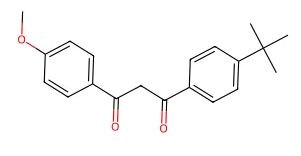
\includegraphics[width=3.3cm]{avobezone.png} & 358~nm & 349~nm \\ \hline
\textcolor{blue}{Ferulic Acid} \newline \texttt{\scriptsize COC1=C(C=CC(=C1)\allowbreak C=CC(=O)O)O} & 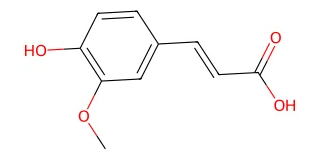
\includegraphics[width=3.3cm]{FerulicAcid.png} & 324~nm & 335~nm \\ \hline
\textcolor{blue}{Homosalate} \newline \texttt{\scriptsize O=C(OC1CC(CC(C1)(C)C)C)\allowbreak c2ccccc2O} & 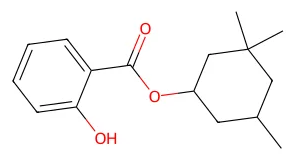
\includegraphics[width=3.3cm]{homosalate.png} & 308~nm & 302~nm \\ \hline
\textcolor{blue}{Octisalate} \newline \texttt{\scriptsize CCCCC(CC)COC(=O)\allowbreak C1=CC=CC=C1O} & 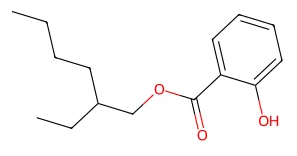
\includegraphics[width=3.3cm]{octisalate.png} & 308~nm & 299~nm \\ \hline
\textcolor{blue}{Oxybenzone} \newline \texttt{\scriptsize O=C(c1ccc(OC)cc1O)\allowbreak c2ccccc2} & 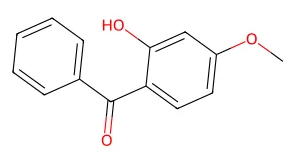
\includegraphics[width=3.3cm]{oxybenzone.png} & 287~nm & 292~nm \\ \hline
\end{longtable}

Prediction errors range from 5~nm (oxybenzone) to 11~nm (ferulic acid), consistent with the overall model RMSE and well within the range useful for screening applications in sunscreen formulation and pharmaceutical photosafety assessment.


\section{Conclusion}

This work presented a comprehensive evaluation of sequential deep learning and classical machine learning approaches for predicting the maximum UV absorption wavelength ($\lambda_{\max}$) of organic molecules from SMILES representations. Using a curated dataset of 18,755 solute--solvent pairs with rigorous stratified cross-validation, we established baseline performance for BiGRU networks (RMSE~$= 36.45 \pm 1.12$~nm, $R^2 = 0.884$) and Random Forest models on Morgan fingerprints (RMSE~$= 32.18 \pm 1.74$~nm, $R^2 = 0.909$).

A central contribution is the solvent-aware SMILES concatenation strategy, where solute and solvent representations are joined with delimiter tokens into a single input sequence. This approach reduces BiGRU prediction error by 3.7\% compared to the solute-only baseline, confirming that solvent effects contribute meaningfully to $\lambda_{\max}$ variability. The strategy requires no handcrafted solvent descriptors and operates end-to-end from raw SMILES.

Cross-dataset benchmarking revealed both the strengths and limitations of 1D SMILES-based models. On the Deep4Chem dataset, our BiGRU achieves RMSE~$= 27.07$~nm, within 2\% of the published GCNN (26.6~nm), demonstrating competitive performance with a simpler architecture. However, scaffold-split evaluation on Jung et al.\ (RMSE~$= 67.56$~nm) and the nablaColors benchmark (RMSE~$= 56.38$~nm vs.\ UniProp MAE~$= 15.97$~nm) highlight that 1D sequence models struggle with structurally novel scaffolds and properties dependent on 3D molecular geometry.

Application to ICH~S10 photosafety classification on a reconstructed Reaxys dataset of 74,784 compounds showed that our RF classifier closely reproduces Mamede et al.'s published results (accuracy 0.879 vs.\ 0.89), validating the practical utility of fingerprint-based approaches for regulatory photosafety screening.

Experimental validation on commercial UV-absorbing compounds---avobenzone ($\Delta = 9$~nm), ferulic acid ($\Delta = 11$~nm), homosalate ($\Delta = 6$~nm), octisalate ($\Delta = 9$~nm), and oxybenzone ($\Delta = 5$~nm)---confirmed that predictions are consistent with the overall model error and useful for screening applications.

\subsection*{Limitations}

Several limitations should be noted: (1)~SMILES representations do not encode 3D conformational information, which is critical for some chromophore classes as demonstrated by the nablaColors gap; (2)~solvents are represented only as SMILES strings, without explicit physical properties such as dielectric constant or hydrogen-bonding capacity; (3)~character-level tokenization may not capture chemically meaningful substructures as effectively as subword or fragment-based tokenization; (4)~the training data is imbalanced across solvents, with common solvents like dichloromethane and chloroform heavily overrepresented.

\subsection*{Future Work}

Several directions emerge from this study. Transfer learning from larger UV absorption databases (e.g., the 92,000-record Reaxys dataset) could improve performance on the primary dataset. Incorporating 3D molecular information, either through geometric descriptors or hybrid 1D/3D architectures, could address the performance gap observed on nablaColors. Attention mechanisms could provide interpretability by identifying key chromophoric substructures. Finally, the trained model can serve as a property filter within generative molecular design pipelines for targeted UV-absorbing molecule discovery.


\section*{Data and Code Availability}
The primary Joung+Beard dataset is available from the Experimental Database of Optical Properties of Organic Compounds \cite{joungExperimentalDatabaseOptical2020}. The Deep4Chem dataset is available on Figshare. The Jung et al.\ dataset is available on GitHub. The nablaColors dataset is available on Zenodo \cite{potapov2026nablacolors}. All code for model training, evaluation, and cross-dataset benchmarking will be made available on GitHub upon publication.

\bibliographystyle{unsrtnat}
\bibliography{Proposal}

% ===== Supplementary Information =====

\end{document}
